\chapter{Analyse et sp\'ecification des besoins}
\section{Introduction}
Ce chapitre est consacr\'e \`a l'analyse et \`a la sp\'ecification des besoins fonctionnels et non fonctionnels de la solution qui est une \'etape primordiale pour la r\'ealisation de notre projet.
\section{Analyse des besoins}
Dans cette partie, nous pr\'esenterons les besoins fonctionnels et non fonctionnels identifi\'es apr\`es la s\'election des besoins.
\subsection{Identification des acteurs}
Dans le cas de notre projet on consid\`ere deux acteurs :
\begin{itemize}
\item \textbf{Le prospecteur} : Il a comme mission principale de g\'erer les anomalies de la plateforme.
\item \textbf{L'exploitant} : Il permet de r\'epondre sur les anomalies qui ne sont pas encore r\'esolu.
\end{itemize}
\subsection{Les besoins fonctionnels}
Au cours de cette \'etape, nous allons extraire les diff\'erentes fonctionnalit\'es offertes par notre projet.
\begin{itemize}
\item L'application prospektor doit permettre \`a chaque prospecteur de :
\begin{itemize}
\item suivre et consulter les anomalies qui a cr\'eer.
\item consulter la liste des attachements li\'ees par anomalies.
\end{itemize}
\item L'application prospektor doit permettre \`a chaque exploitant de :
\begin{itemize}
\item suivre et consulter les anomalies par \'etape, date \& criticit\'e.
\item consulter les attachements li\'ees par anomalies.
\item Ajouter des attachements aux anomalies qui ne sont pas encore r\'esolu.
\end{itemize}  
\end{itemize}

\subsection{Description des cas d'utilisation}
Cette figure repr\'esente le diagramme de cas d'utilisation globale de l'acteur prospecteur :
\begin{figure}[H]
	\center{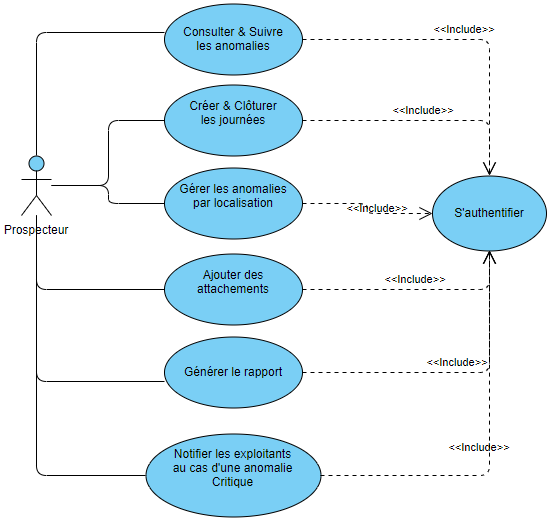
\includegraphics[width=\textwidth]{Figures/prospectorDiagram.png}}
	\caption{\label{fig:my-label} Diagramme de cas d'utilisation globale pour le prospecteur}
\end{figure}

Cette figure repr\'esente le diagramme de cas d'utilisation globale de l'acteur exploitant :
\begin{figure}[H]
	\center{\includegraphics[width=\textwidth]{Figures/exploitantDiagram.png}}
	\caption{\label{fig:my-label} Diagramme de cas d'utilisation globale pour l'exploitant}
\end{figure}

\subsection{Les besoins non fonctionnels}
Outre les fonctions cit\'ees ci-dessus, l'application doit assurer en certaine mesure les caract\'eristiques suivantes :
\begin{itemize}
\item L'efficacit\'e : L'efficacit\'e de l'application doit permettre l'accomplissement de la t\^ache avec le minimum de manipulation. Ceci doit \^etre garanti pour que l'application puisse s'int\'egrer facilement dans l'environnement ou elle va \^etre d\'eploy\'ee.

\item La s\'ecurit\'e : Les diff\'erents comptes utilis\'es par les utilisateurs doivent \^etre s\'ecuris\'es et v\'erifi\'es pour \'eviter les faux comptes et les fausses informations.

\item La fiabilit\'e : Touche \`a l'aspect qualit\'e des donn\'ees et persistance des informations dans l'application ainsi que la vitesse de chargement des interfaces.
\end{itemize} 

Aussi l'application doit fonctionner d'une fa\c{c}on coh\'erente sans erreur








On a dr\'esse le RoadMap qui va \^etre r\'ealiser entre Mars et Juin.

\begin{figure}[!htb]
	\center{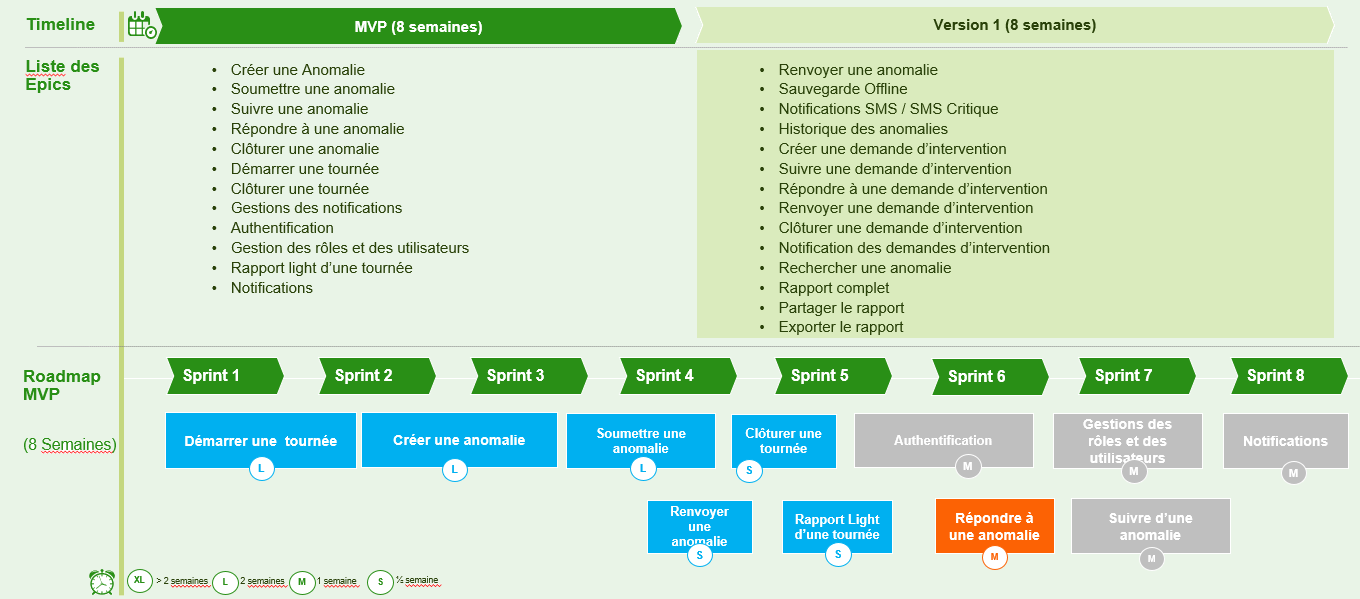
\includegraphics[width=\textwidth]{Figures/roadmap.png}}
	\caption{\label{fig:my-label} RoadMap du projet}
\end{figure}


\subsection{Description des cas d'utilisation}
\section{Conclusion}